\documentclass[10pt,a4paper,landscape]{article}
% -- Layout ----
\usepackage[top=0.6cm, bottom=0.6cm, left=0.5cm, right=0.5cm, landscape]{geometry}

% -- Titles ----
\usepackage[
  tiny,                     % text size title
  compact                   % reduce vertical space before/after title
]{titlesec}
% \titlespacing*
\titleformat{\section}{\normalfont\small\bfseries}{\thesection}{0em}{} % Remove space before and after section titles
\titleformat{\subsection}{\normalfont\small\bfseries}{\thesubsection}{0em}{} % Remove space before and after subsection titles
\titlespacing*{\section}{0pt}{0pt}{0pt} % Remove space before/after section titles
\titlespacing*{\subsection}{0pt}{0pt}{0pt} % Remove space before/after subsec titles

% -- Colors ----
\usepackage[dvipsnames]{xcolor}
\definecolor{dmm}{RGB}{192,192,192} % Define a custom dimmed text color
\definecolor{cmt}{RGB}{61,123,123}

% -- Math ------
\usepackage{mathtools}
\usepackage{amssymb}
\usepackage{turnstile}%better vdash

% -- Lists -----
\usepackage[inline]{enumitem}
\setlist{noitemsep}% Remove vspace between items
% Set vspace before and after  list environments as well as the left margin
\setlist[itemize,1]{leftmargin=.6em,labelindent=0pt,labelsep=2pt,
  topsep=1pt,partopsep=1pt}
\setlist[enumerate,1]{leftmargin=1em,labelindent=0pt,labelsep=2pt,
  topsep=1pt,partopsep=1pt}
\setlist[itemize,2]{leftmargin=.3em,labelindent=1pt,topsep=1pt,partopsep=1pt}
\setlist[enumerate,2]{leftmargin=0.2em,labelindent=1pt,topsep=1pt,partopsep=1pt}
\setlist[description]{labelwidth=\linewidth,font=\small\bfseries,leftmargin=1em,topsep=1pt,partopsep=1pt}
% -- Code listing ---
\usepackage{listings}
\lstset{
  aboveskip=3pt,
  belowskip=3pt,
  basicstyle=\small\ttfamily,
  breaklines=true,
  % commentstyle=\upshape\ttfamily,
  captionpos=b,
  commentstyle=\color{cmt},
  columns=flexible,
  frame=single,
  keepspaces=false,
  keywordstyle=\bfseries,
  showspaces=false,
  showstringspaces=false,
  showtabs=false,
  tabsize=2,
}

% Parse Trees
\usepackage{tikz}
\usetikzlibrary{ arrows, automata, bbox, calc, positioning, tikzmark, decorations.pathmorphing, decorations.pathreplacing, decorations.shapes, }
\tikzset{
  >=stealth',
  node distance=1cm,
  recstate/.style={
    circle,draw=blue!50,fill=blue!20,thick,font=\small\sffamily,rounded corners=3pt,
    minimum size=1cm,inner sep=1pt
  },
  ivp/.style={draw,->,auto,font=\small\sffamily,bend angle=60},
  msi/.style={draw=Brown,->,auto,font=\small\sffamily,bend angle=80},
  msibs/.style={draw=RoyalBlue,->,auto,font=\small\sffamily,bend angle=80},
  msinl/.style={font=\footnotesize\sffamily}, %msi node label
  every edge/.style={draw,auto,font=\small\sffamily},
  every loop/.style={looseness=4},
  initial text=start,initial where=right
}

% Place a figure env right here via [H] option
\usepackage{float}

% Side by side figure
\usepackage{subcaption}
% \usepackage{caption}
% \captionsetup{belowskip=0pt, aboveskip=0pt}
\usepackage{pifont}

% -- Multi-Col layout --
\usepackage{multicol}

% No indentation
\setlength\parindent{0pt}
\setlength\abovedisplayskip{-5pt}
\setlength\belowdisplayskip{-5pt}
\setlength\abovedisplayshortskip{-4pt}
\setlength\belowdisplayshortskip{-4pt}
\setlength\tabcolsep{5pt}
\newcommand{\gor}{\;|\;}
\newcommand{\num}{\texttt{\#}~}
\newcommand{\pro}[1]{\textcolor{Brown}{#1}}
\newcommand{\bus}[1]{\textcolor{RoyalBlue}{#1}}
\renewcommand{\arraystretch}{1.2}


\begin{document}
% Suppress page number for all pages
\pagestyle{empty}

% Each section goes into this env
\begin{multicols*}{3}
\section*{LR(0) item, closure, goto}
\begin{itemize}
\item \mb{item}: a grammar rule with a dot(\textbf{.}) that indicates a
  parser position in its RHS: $A \to \alpha\beta\gamma$ thus can have the following:
  \begin{align*}
    A &\to \lrd\alpha\beta\gamma \\
    A &\to \alpha\lrd\beta\gamma \\
    A &\to \alpha\beta\lrd\gamma \\
    A &\to \alpha\beta\gamma\lrd
  \end{align*}
\item $X \to\varepsilon$ has its own item: $X\to\lrd$
\item When dot already at the end, no change to the item $X\to A\lrd$
\item \mb{closure}: for item $A\to\alpha\lrd B\beta$ where $B$ is a \mo{non-terminal}. If $B$ has multiple productions $B\to \gamma_1 \gor \cdots \gor \gamma_n$, then \mo{all} $B\to\lrd\gamma_i\;(1 \leq i \leq n)$ should be in the same state as the item
\item \mb{goto}: for item $A\to\alpha\lrd X\beta$ where $X$ can be a terminal or non-terminal, then create a new state that must contains
  \begin{enumerate}
  \item item $A\to\alpha X\lrd\beta$ (i.e. pass $X$), plus
  \item the closure of the above item
  \end{enumerate}
\item \textbf{closure} is about adding new \textbf{items} to a LR(0) DFA state
\item \textbf{goto} is about creating transitions and states in LR(0) DFA
\end{itemize}
\section*{Example: create LR(0) DFA (parsing table and states)}
\begin{align*}
  S&\to (L)   \tag{1} \\
  S&\to x     \tag{2} \\
  L&\to S     \tag{3} \\
  L&\to L,S   \tag{4}
\end{align*}

\section*{Step 1: Augment the grammar to include a start symbol}
\begin{align*}
  S'&\to S\$  \tag{0} \\
  S&\to (L)   \tag{1} \\
  S&\to x     \tag{2} \\
  L&\to S     \tag{3} \\
  L&\to L,S   \tag{4}
\end{align*}
Also if there is any rule like $X\to N_1 \gor N_2 \dots$, rewrite it to
\begin{align*}
  X\to N_1 & X\to N_2 \cdots
\end{align*}
\section*{Step 2: Create start state for LR(0) DFA}
\begin{enumerate}
\item start with \textbf{starting item} $S'\to \lrd S\$$ and create state 1
  \begin{center}
    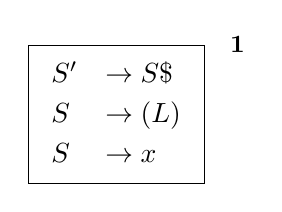
\begin{tikzpicture}[state/.style=draw]
    \node (s1) [state] {
      \begin{tabular}{ll}
         $S'$ & $\to\lrd S\$$  \\
         $S$  & $\to\lrd (L)$  \\
         $S$  & $\to\lrd x$
      \end{tabular}
    };
    \node (m1) [right=2mm of s1.north east,font=\bf\small]{1};
    \end{tikzpicture}
  \end{center}
\item there is no non-terminals before \mr{\textbf{.}} so need \textbf{goto}
\item In state 1, use goto to create edges and new states
  \begin{itemize}
  \item \textbf{goto}($x$) $\Rightarrow$ state 2
  \end{itemize}
  \begin{center}
    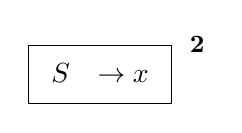
\begin{tikzpicture}[state/.style=draw]
      \node (s2) [state] {
        \begin{tabular}{ll}
          $S$ & $\to x\lrd$
        \end{tabular}
      };
      \node (m2) [right=1mm of s2.north east,font=\bf\small]{2};
    \end{tikzpicture}
  \end{center}
  \begin{itemize}
  \item \textbf{goto}(left-paren) $\Rightarrow$ state 3
  \end{itemize}
  \begin{center}
    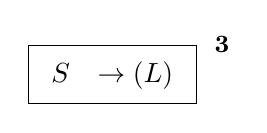
\begin{tikzpicture}[state/.style=draw]
      \node (s3) [state] {
        \begin{tabular}{ll}
          $S$ & $\to (\lrd L)$
        \end{tabular}
      };
      \node (m3) [right=1mm of s3.north east,font=\bf\small]{3};
    \end{tikzpicture}
  \end{center}
\item In state 3, $L$ is a non-terminal so need to add \textbf{closure}($L$)
\item[] Similarly, $S$ is a non-termina so need to add \textbf{closure}($S$) when done with $L$. Last two items also appear in state 1
  \begin{center}
    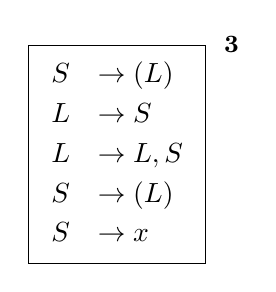
\begin{tikzpicture}[state/.style=draw]
    \node (s3) [state] {
      \begin{tabular}{ll}
         $S$ & $\to (\lrd L)$ \\
         $L$ & $\to \lrd S$ \\
         $L$ & $\to \lrd L,S$ \\
         $S$ & $\to \lrd (L)$ \\
         $S$ & $\to \lrd x$ \\
      \end{tabular}
    };
    \node (m3) [right=1mm of s3.north east,font=\bf\small]{3};
    \end{tikzpicture}
  \end{center}
\item In state 1, \textbf{goto}($S$) and get state 4
  \begin{center}
    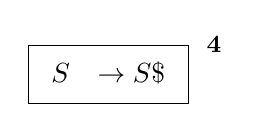
\begin{tikzpicture}[state/.style=draw]
    \node (s4) [state] {
      \begin{tabular}{ll}
         $S$ & $\to S\lrd\$$
      \end{tabular}
    };
    \node (m4) [right=1mm of s4.north east,font=\bf\small]{4};
    \end{tikzpicture}
  \end{center}
\item In state 3, closure is done, we need goto (start with easy)
  \begin{itemize}
  \item \textbf{goto}($x$), item $S\to x\lrd \Rightarrow$ existing state 2
  \item \textbf{goto}(\textsf{left-pare}), item $S\to (\lrd L)\Rightarrow$ existing state 3
  \item \textbf{goto}($L$), item $S\to (L\lrd)\Rightarrow$ new state 5
  \item \textbf{goto}($L$), item $L\to L\lrd,S\Rightarrow$ new state 5
  \begin{center}
    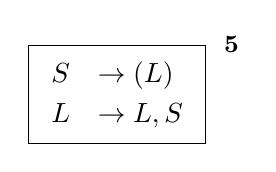
\begin{tikzpicture}[state/.style=draw]
    \node (s5) [state] {
      \begin{tabular}{ll}
         $S$ & $\to (L\lrd)$ \\
         $L$ & $\to L\lrd,S$
      \end{tabular}
    };
    \node (m5) [right=1mm of s5.north east,font=\bf\small]{5};
    \end{tikzpicture}
  \end{center}
  \item \textbf{goto}($S$), item $L\to S\lrd\Rightarrow$ new state 7
  \begin{center}
    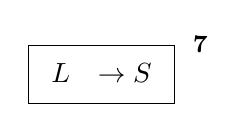
\begin{tikzpicture}[state/.style=draw]
    \node (s7) [state] {
      \begin{tabular}{ll}
         $L$ & $\to S\lrd$
      \end{tabular}
    };
    \node (m7) [right=1mm of s7.north east,font=\bf\small]{7};
    \end{tikzpicture}
  \end{center}
  \end{itemize}
\item In state 5, need \textbf{goto} as there's no closure to be computed
  \begin{itemize}
  \item \textbf{goto}(\textsf{right-paren}), item $S\to (L)\lrd \Rightarrow$ new state 6
    \begin{center}
      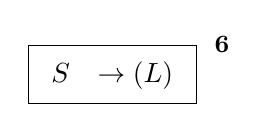
\begin{tikzpicture}[state/.style=draw]
        \node (s6) [state] {
          \begin{tabular}{ll}
            $S$ & $\to (L)\lrd$
          \end{tabular}
        };
        \node (m6) [right=1mm of s6.north east,font=\bf\small]{6};
      \end{tikzpicture}
    \end{center}
  \item \textbf{goto}(,), item $L\to L,\lrd S \Rightarrow$ new state 8
    \begin{center}
      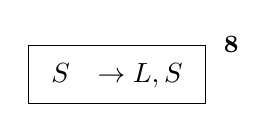
\begin{tikzpicture}[state/.style=draw]
        \node (s8) [state] {
          \begin{tabular}{ll}
            $S$ & $\to L,\lrd S$
          \end{tabular}
        };
        \node (m8) [right=1mm of s8.north east,font=\bf\small]{8};
      \end{tikzpicture}
    \end{center}
  \end{itemize}
\item In state 8, $S$ is non-terminal so need add \textbf{closure}($S$)
  \begin{center}
    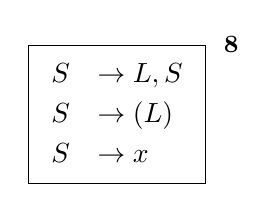
\begin{tikzpicture}[state/.style=draw]
      \node (s8) [state] {
        \begin{tabular}{ll}
          $S$ & $\to L,\lrd S$ \\
          $S$ & $\to \lrd(L)$ \\
          $S$ & $\to \lrd x$
        \end{tabular}
      };
      \node (m8) [right=1mm of s8.north east,font=\bf\small]{8};
    \end{tikzpicture}
  \end{center}
\item In state 8, now apply goto rule:
  \begin{itemize}
  \item \textbf{goto}($S$), item $S\to (L,S)\lrd \Rightarrow$ new state 9
    \begin{center}
      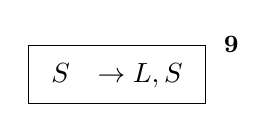
\begin{tikzpicture}[state/.style=draw]
        \node (s9) [state] {
          \begin{tabular}{ll}
            $S$ & $\to L,S\lrd$ \\
          \end{tabular}
          % $S\to (L,S)\lrd$
        };
        \node (m9) [right=1mm of s9.north east,font=\bf\small]{9};
      \end{tikzpicture}
    \end{center}
  \item \textbf{goto}(\textsf{left-paren}), item $S\to (\lrd L) \Rightarrow$ existing state 3
  \item \textbf{goto}($x$), item $S\to x\lrd \Rightarrow$ existing state 2
  \end{itemize}
\end{enumerate}
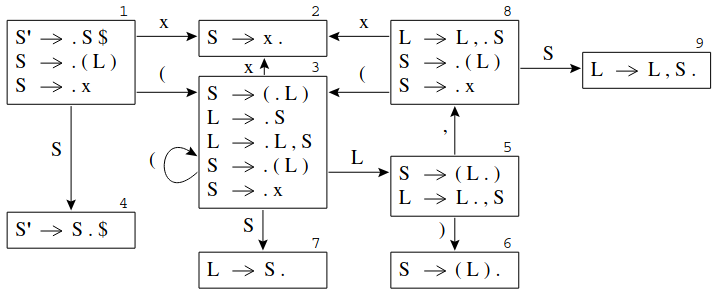
\includegraphics[width=\linewidth]{img/LR0}
\section*{Step 3: draw parse table (row is state, col is symbol)}

\begin{itemize}
\item In edege $I\overset{X}{\to} J$, if $X$ is \mb{terminal}, \emph{shift} $J$ at $(I,X)$
\item In edege $I\overset{X}{\to} J$, if $X$ is \mb{non-terminal}, \emph{goto} $J$ at $(I,X)$
\item For each $I$ with an item $S'\to S\lrd\$$, \mb{accept} at $(I,\$)$
\item For any $I$ with item $A\to \gamma\lrd$, \mb{reduce $n$} ($n$ is this production's num in the grammar) at $(I,Y)$ for every $Y$
\end{itemize}
\begin{tabular}{r|lllll|ll}
  state $I$& (   & )   & $x$ &,    & $\$$ & $S$  & $L$ \\
  \hline
  1        &$s3$ &     &$s2$ &     &      & $g4$ &      \\
  2        &$r2$ &$r2$ &$r2$ &$r2$ & $r2$ &      &      \\
  3        &$r3$ &     &$r2$ &     &      & $g7$ & $g5$ \\
  4        &     &     &     &     & $a$  &      &    \\
  5        &     &$s6$ &     &$s8$ &      &      &    \\
  6        &$r1$ &$r1$ &$r1$ &$r1$ &$r1$  &      &    \\
  7        &$r3$ &$r3$ &$r3$ &$r3$ &$r3$  &      &    \\
  8        &$s3$ &     &$s2$ &     &      & $g9$ &    \\
  9        &$r4$ &$r4$ &$r4$ &$r4$ &$r4$  &      &    \\
  \hline
\end{tabular}
\end{multicols*}
\end{document}
